\documentclass[11pt]{article}
\usepackage[paper=letterpaper,margin=2cm]{geometry}
\usepackage{graphicx}
\usepackage{hyperref}
\usepackage{enumitem}
\usepackage{amsmath,amsfonts,amssymb}
\usepackage{todonotes}
\usepackage[export]{adjustbox}
\usepackage{wrapfig}

\graphicspath{ {./images/} }

\hypersetup{
    colorlinks,
    citecolor=black,
    filecolor=black,
    linkcolor=black,
    urlcolor=black
}

\setuptodonotes{color=blue!15}

\setlength\parskip{1em plus 0.1em minus 0.2em}
\setlength{\parindent}{0pt}

\newcommand{\twopartdef}[4]
{ \displaystyle
	\left\{
		\begin{array}{ll}
			#1 & \mbox{se } #2 \\
			#3 & \mbox{se } #4
		\end{array}
	\right.
}

\newcommand{\threepartdef}[6]
{ \displaystyle
	\left\{
		\begin{array}{ll}
			#1 & \mbox{se } #2 \\
			#3 & \mbox{se } #4 \\
            #5 & \mbox{se } #6
		\end{array}
	\right.
}

\begin{document}

\begin{titlepage}
    \begin{center}
        \vspace*{1cm}

        \textbf{\LARGE Análise e Síntese de Algoritmos}
        \vspace{0.5cm}

        \Large Resumo
        \vspace{1.5cm}

        \textbf{Rafael Rodrigues}
        \vfill
        LEIC \\
        Instituto Superior Técnico \\
        2023/2024
    \end{center}
\end{titlepage}

\tableofcontents

\newpage

\section{Fundamentos} \todo{Slides Aula 1 e 2}

\subsection{Divide-and-Conquer}

\begin{itemize}
    \item Dividir o problema num conjunto de sub-problemas do mesmo tipo.
    \item Resolver cada sub-problema (com uma chamada recursiva).
    \item Combinar as soluções dos sub-problemas para obter a solução do
          problema original.
\end{itemize}

\subsection{Teorema Mestre}

\subsubsection{Teorema Mestre Simplificado}

Se \ $T(n) = aT(n/b) + n^d$ , \ $a \ge 1$, \ $b > 1$, \ $d \ge 0$ , então:

\begin{equation*}
    T(n) = \threepartdef{O(n^d)}{d > \log_ba}
    {O(n^d \log_bn)}{d = \log_ba}
    {O(n^{\log_ba})}{d < \log_ba}
\end{equation*}

\subsubsection{Teorema Mestre Generalizado}

Se \ $T(n) = aT(n/b) + f(n)$ , \ $a \ge 1$, \ $b > 1$ , então:

\begin{equation*}
    T(n) = \threepartdef{\Theta(n^{\log_ba})}{f(n) = O(n^{\log_ba-\varepsilon})}
    {\Theta(n^{\log_ba} \log n)}{f(n) = \Theta(n^{\log_ba})}
    {\Theta(f(n))}{f(n) = \Omega(n^{\log_ba+\varepsilon})}
\end{equation*}

\newpage

\section{Sorting and Order Statistics}

\subsection{Amontoados} \todo{Slides Aula 5}

Um \textbf{heap} é um vetor de valores ($A$) interpretado como uma árvore binária (essencialmente completa), em que $A[1]$ é a raíz da árvore e $A[Parent(i)] \ge A[i]$.

\begin{minipage}{0.4\textwidth}
    Relações entre nós da árvore:
    \begin{itemize}
        \item Parent($i$) = $\lfloor i/2 \rfloor$
        \item Left($i$) = $2i$
        \item Right($i$) = $2i + 1$
    \end{itemize}
\end{minipage}
\begin{minipage}{0.59\textwidth}
    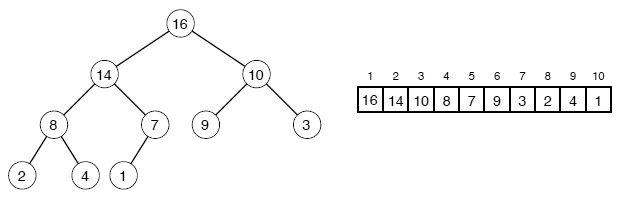
\includegraphics[scale=0.7, right]{heap.png}
\end{minipage}

\subsubsection{Operações sobre Amontoados}

\begin{itemize}[topsep=0pt]
    \item \textbf{Max-Heapify($A,\ i$)}: $O(\log n)$
          \begin{itemize}[topsep=0pt]
              \item Transforma a árvore com raiz em $i$ num amontoado, assumindo que as árvores com raiz em Left($i$) e Right($i$) são amontoados
          \end{itemize}
    \item \textbf{Build-Max-Heap($A$)}: $O(n)$
          \begin{itemize}[topsep=0pt]
              \item Construir amontoado a partir de um vector arbitrário
              \item Chamada seletiva de Max-Heapify
          \end{itemize}
\end{itemize}

\subsubsection{Algoritmo Heap-Sort}

\begin{enumerate}
    \item Extrair consecutivamente o elemento máximo de uma heap
    \item Colocar esse elemento na posição (certa) do vector
\end{enumerate}
\begin{itemize}[topsep=0pt]
    \item \textbf{Complexidade}: $O(n \log n)$
\end{itemize}

\subsubsection{Outras Operações}

\begin{itemize}[topsep=0pt]
    \item \textbf{Heap-Maximum($A$)}: $O(1)$
          \begin{itemize}[topsep=0pt]
              \item Devolve o maior elemento da heap
          \end{itemize}
    \item \textbf{Heap-Extract-Max($A$)}: $O(\log n)$
          \begin{itemize}[topsep=0pt]
              \item Remove o maior elemento da heap
          \end{itemize}
    \item \textbf{Heap-Increase-Key($A,\ i ,\ key$)}: $O(\log n)$
          \begin{itemize}[topsep=0pt]
              \item Incrementa o elemento $i$ para o valor $key$
          \end{itemize}
    \item \textbf{Max-Heap-Insert($A,\ key$)}: $O(\log n)$
          \begin{itemize}[topsep=0pt]
              \item Insere $key$ na heap
          \end{itemize}
\end{itemize}

\newpage

\setcounter{section}{3}

\section{Técnicas de Síntese de Algoritmos}

\subsection{Programação Dinâmica} \todo{Slides Aula 3 e 4}

Passos para a realização de um algoritmo baseado em programação dinâmica:
\begin{itemize}[topsep=0pt]
    \item Caracterizar \textbf{estrutura} de uma solução ótima
    \item Definir \textbf{recursivamente} o valor de uma solução ótima
    \item Calcular valor da solução ótima utilizando abordagem \textbf{bottom-up}
    \item Construir \textbf{solução} a partir da informação obtida
\end{itemize}

\vspace{8pt}

Características da Programação Dinâmica:
\begin{itemize}[topsep=0pt]
    \item Solução ótima do problema composta por soluções ótimas para sub-problemas
    \item Solução construtiva para evitar resolver repetidamente o mesmo problema
          \begin{itemize}
              \item Solução recursiva resolve repetidamente os mesmos sub-problemas
          \end{itemize}
    \item Reconstrução da solução ótima
    \item Memorização
          \begin{itemize}
              \item Permite obter tempo de execução das soluções bottom-up, mas
                    utilizando abordagem recursiva, \textbf{memorizando} resultados de sub-problemas já resolvidos
          \end{itemize}
\end{itemize}

\newpage

\subsection{Algoritmos Greedy} \todo{Slides Aula 6}

Caracteristicas Algoritmos Greedy
\begin{itemize}[topsep=0pt]
    \item \textbf{Propriedade da escolha greedy}
          \begin{itemize}
              \item Ótimo (global) para o problema pode ser encontrado realizando escolhas locais ótimas (em programação dinâmica, esta escolha está dependente de resultados de sub-problemas)
          \end{itemize}
    \item \textbf{Sub-estrutura ótima}
          \begin{itemize}
              \item Solução ótima do problema engloba soluções ótimas para sub-problemas
          \end{itemize}
\end{itemize}

\subsubsection{Seleção de Atividades}

A escolha greedy é optar sempre pela \textbf{próxima atividade que acabar mais cedo}.

\subsubsection{Algoritmo de Huffman}

\begin{enumerate}
    \item Adicionar cada caracter à fila de prioridade, pela ordem ascendente de frequência.
    \item Retirar os dois elementos com menor frequência da fila.
    \item Somam-se os valores dos dois elementos, criando um novo nó com esse valor, que é inserido na fila.
    \item Enquanto a fila não estiver vazia, voltar ao passo 2.
    \item Numerar os nós de acordo com o enunciado.
\end{enumerate}

Custo do código de uma árvore binário $T$, sobre um alfabeto $\Lambda $:
\begin{equation*}
    B(T)=\sum_{i \in \Lambda} f(i) \cdot d_T(i)\ ,\ d_T\ \text{corresponde à profundidade de } i\ \text{na árvore binária}
\end{equation*}
A frequência pode corresponder a uma fração do número total de caracteres, neste caso:
\begin{equation*}
    \text{Total Bits} =
    B(T)\times\frac{\text{\#caracteres}}{\text{raiz da árvore}\ T}
\end{equation*}

\newpage

\subsection{Análise Amortizada} \todo{Slides Aula 7 e 8}

\textbf{Análise Amortizada} - Determina o \textbf{custo médio} de uma \textbf{sequência de operações} sobre uma estrutura de dados.

\textbf{Custo Amortizado} - Dada uma sequência de n operações com uma complexidade total de $T(n)$, o custo amortizado de cada operação é $T(n)/n$

\vspace{8pt}

\textbf{Métodos para Análise Amortizada:}
\begin{itemize}[topsep=0pt]
    \item Método de análise agregada
          \begin{itemize}[topsep=0pt]
              \item Determina o custo amortizado de uma sequência de operações
              \item Divide o custo total $T(n)$ pelo número de $n$ operações
          \end{itemize}
    \item Método do contabilista
          \begin{itemize}[topsep=0pt]
              \item Mais que um tipo de operação, cada operação tem custo \textbf{real} e custo \textbf{amortizado}
              \item Operações baratas \textbf{pagam mais} para que operações caras \textbf{paguem menos}
          \end{itemize}
    \item Método do potencial
          \begin{itemize}[topsep=0pt]
              \item Variação do método do contabilista, onde o crédito pago a mais por certas operações é mantido como \textbf{energia potencial} total que pode ser gasto em operações caras
          \end{itemize}
\end{itemize}

\newpage

\section{Estruturas de Dados Avançadas}

\subsection{Estrutura de Dados para Conjuntos Disjuntos} \todo{Slides Aula 14}

Operações sobre Conjuntos Disjuntos:
\begin{itemize}[topsep=0pt]
    \item \textbf{Make-Set($x$)} - Cria novo conjunto que apenas inclui o elemento $x$, que será o representante do conjunto.
    \item \textbf{Find-Set($x$)} - Retorna o representante do conjunto que contém $x$.
    \item \textbf{Union($x,y$)} - Realiza a união dos conjuntos que contêm $x$ e $y$, respetivamente $S_x$ e $S_y$.
\end{itemize}

\subsubsection{Estruturas Baseadas em Listas}

\begin{minipage}{0.55\textwidth}
    \begin{itemize}[topsep=0pt]
        \item Cada conjunto representado por uma lista ligada.
        \item Primeiro elemento é o representante do conjunto.
        \item Todos os elementos incluem apontador para o representante do conjunto.
    \end{itemize}
\end{minipage}
\begin{minipage}{0.44\textwidth}
    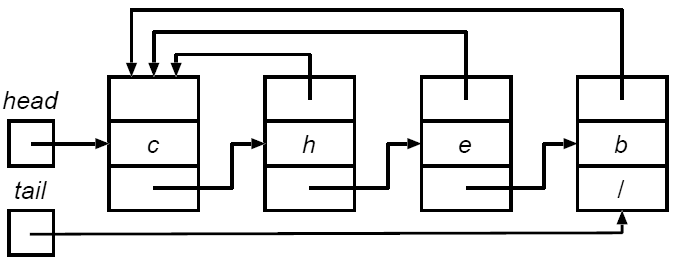
\includegraphics[scale=0.4,right]{linked_list.png}
\end{minipage}

\textbf{Heurística União Pesada} \\[6pt]
Associa a cada conjunto o seu número de elementos, permitindo juntar a lista com menor número de elementos à lista com maior número de elementos em cada operação Union.

\textbf{Complexidade}: $O(m+n\log n)$ para $m$ operações com $n$ Union

\subsubsection{Estruturas Baseadas em Árvores}

\begin{itemize}
    \item Cada conjunto representado por uma árvore.
    \item Cada elemento aponta apenas para antecessor na árvore.
    \item Representante da árvore é a raiz, que antecede a si própria.
\end{itemize}

\textbf{Heurística de União por Categoria} \\[6pt]
O representante de cada conjunto guarda a sua categoria (rank), que inicialmente é 0. O rank pode ser aumentado quando há uma união de dois conjuntos, onde se coloca a árvore com menor rank a apontar para árvore com maior rank. Utilizando apenas esta heurística a \textbf{complexidade} é $O(m\cdot\log n)$.

\begin{minipage}{0.50\textwidth}
    \textbf{Heurística de Compressão de Caminhos} \\[6pt]
    Em cada operação Find-Set coloca cada nó visitado a apontar diretamente para a raiz da árvore
\end{minipage}
\begin{minipage}{0.49\textwidth}
    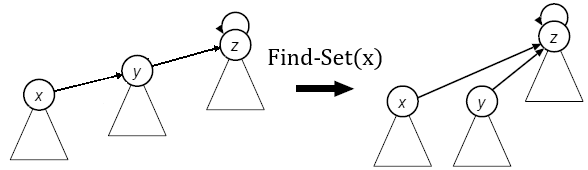
\includegraphics[scale=0.5,right]{three_heuristic_2.png}
\end{minipage}

\textbf{Complexidade}: $O(m\cdot\alpha(n)) \approx O(m)$ para $m$ operações com $n$ Union

\newpage

\section{Algoritmos em Grafos}

\subsection{Algoritmos Elementares} \todo{Slides Aula 9 e 10}

\subsubsection{Representação de Grafos}

Dado um grafo $G = (V,E)$, um \textbf{caminho} $p$ é uma sequência $\langle v_0,v_1, \ldots,v_k \rangle$ tal que para todo o $i,\ 0 \le i \le k-1, (v_i ,v_{i+1}) \in E$.
\begin{itemize}[topsep=0pt]
    \item Se existe um caminho $p$ de $u$ para $v$, então $v$ diz-se \textbf{atingível} a partir de $u$ usando $p$.
    \item Um \textbf{ciclo} num grafo $G = (V,E)$ é um caminho $\langle v_0,v_1, \ldots,v_k \rangle$, tal que $v_0 = v_k$.
    \item Um grafo dirigido $G = (V,E)$ diz-se \textbf{acíclico} (ou Directed Acyclic Graph (DAG)) se não tem ciclos.
\end{itemize}

\subsubsection{Breadth-First Search}

Dados $G = (V,E)$ e vértice fonte $s$, o algoritmo BFS explora
sistematicamente os vértices de $G$ para descobrir todos os vértices
atingíveis a partir de $s$.

\textbf{Árvore Breadth-First} - é um sub-grafo de $G$, inclui todos os vértices atingíveis a partir de $s$ e os arcos que definem a relação predecessor da BFS.

\subsubsection{Depth-First Search}

\todo[inline]{DFS}

\subsubsection{Ordenação Topológica}

Uma \textbf{ordenação topológica} de um DAG $G = (V,E)$ é uma ordenação de
todos os vértices tal que se $(u,v) \in E$ então $u$ aparece antes de $v$ na
ordenação.

Complexidade: $O(V+E)$

\subsubsection{Componentes Fortemente Ligados}

Dado um grafo dirigido $G = (V,E)$ um \textbf{componente fortemente ligado} (ou Strongly Connected Component (SCC)) é um conjunto máximo de vértices $U \subseteq V$, tal que para quaisquer $u,\ v \in U$, $u$ é atingível a partir de $v$, e $v$ é atingível a partir de $u$.

Complexidade: $O(V+E)$

\subsection{Árvores Abrangentes de Menor Custo} \todo{Slides Aula 13}

\begin{itemize}[topsep=0pt]
    \item Um grafo não dirigido $G = (V,E)$, diz-se \textbf{ligado} se para qualquer par de vértices existe um caminho que liga os dois vértices
    \item Dado um grafo não dirigido $G = (V,E)$, ligado, uma \textbf{árvore abrangente} é um sub-conjunto acíclico $T \subseteq E$, que liga todos os vértices
    \item O tamanho da árvore é $|T| = |V| - 1$
    \item Uma \textbf{árvore abrangente de menor custo} é uma árvore abrangente $T$ em que a soma dos pesos dos seus arcos é minimizada.
          \begin{equation*}
              \min w(T)=\sum_{(u,v)\in T} w(u,v)
          \end{equation*}
\end{itemize}

\subsubsection{Algoritmo de Prim}

\begin{minipage}{0.65\textwidth}
    \begin{enumerate}
        \item Escolher um vértice raiz $r$ (que passa a ser a árvore) e adicionar os restantes vértices à fila por explorar.
        \item Procurar o arco adjacente de menor peso que liga a árvore a um vértice não explorado. Adicionar esse arco à árvore e remover o vértice da fila por explorar.
        \item Cada vértice guarda o seu antecessor, $\pi[v]$, e o peso do arco que o liga à árvore, $key[v]$.
        \item Voltar ao segundo passo até não haver vértices por explorar.
    \end{enumerate}
    \begin{itemize}
        \item \textbf{Complexidade}: $O(E \cdot \log V)$
    \end{itemize}
\end{minipage}
\begin{minipage}{0.34\textwidth}
    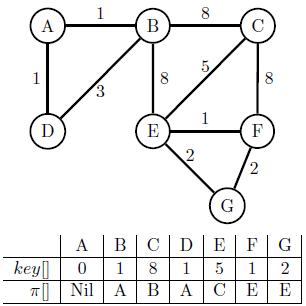
\includegraphics[scale=0.7, right]{prim.png}
\end{minipage}

\subsubsection{Algoritmo de Kruskal}

\begin{enumerate}
    \item Cria uma floresta de árvores, em que cada vértice é uma árvore. (\textbf{Make-Set})
    \item Percorre as arestas do grafo pela ordem ascendente de peso.
    \item Para cada aresta verifica se os seus vértices pertencem a árvores diferentes. (\textbf{Find-Set})
    \item Se sim, une as duas árvores. (\textbf{Union})
\end{enumerate}
\begin{itemize}[topsep=0pt]
    \item \textbf{Complexidade}: $O(E \cdot \log V)$ \\[8pt]
          Esta complexidade é obtida recorrendo às estruturas de dados adequadas, referidas no \hyperlink{section.5}{\underline{Capítulo 5}}
\end{itemize}

\newpage

\subsection{Caminhos Mais Curtos com Fonte Única} \todo{Slides Aula 11}

\begin{itemize}
    \item Dado um grafo $G = (V,E)$, dirigido, com uma função de pesos $w : E \rightarrow \mathbb{R}$, define-se o \textbf{peso de um caminho} $p$, onde $p=\langle v_0,v_1, \ldots,v_k \rangle $, como a soma dos pesos dos arcos que compõem $p$:
          \begin{equation*}
              w(p) = \sum_{i=1}^{k} w(v_{i-1},v_i)
          \end{equation*}
    \item O \textbf{peso do caminho mais curto} de $u$ para $v$ é definido por:
          \begin{equation*}
              \delta(u,v) = \twopartdef{min\{w(p): u \rightarrow_p v\}}
              {\text{existe caminho de u para v}}
              {\infty}{\text{não existe}}
          \end{equation*}
    \item Um \textbf{caminho mais curto} de $u$ para $v$ é qualquer caminho $p$ tal que $w(p) = \delta(u,v)$.
\end{itemize}

\subsubsection{Algoritmo Dijkstra}

\begin{enumerate}
    \item Mantém conjunto de vértices $S$ com pesos dos caminhos mais curtos já calculados
    \item A cada passo seleciona vértice $u \in V-S$ com menor estimativa do peso do caminho mais curto
    \item Insere o vértice $u$ em $S$ e relaxa os arcos que saem de $u$
\end{enumerate}
\begin{itemize}[topsep=0pt]
    \item Só permite \textbf{pesos não negativos}.
    \item \textbf{Complexidade}: $O((V+E)\log V)$
\end{itemize}

\subsubsection{Algoritmo Bellman-Ford}

\begin{enumerate}
    \item Relaxa todas as arestas do grafo $V-1$ vezes, com vista a atualizar gradualmente a estimativa de custo associado a cada vértice.
    \item Percorre mais uma vez todas as arestas, de modo a verificar se há algum ciclo negativo.
\end{enumerate}
\begin{itemize}[topsep=0pt]
    \item Permite \textbf{pesos negativos} e identifica \textbf{ciclos negativos}.
    \item \textbf{Complexidade}: $O(VE)$
\end{itemize}

\subsubsection{Caminhos mais curtos em DAGs}

\begin{enumerate}
    \item Ordena os vértices do grafo pela ordem topológica.
    \item Relaxa os vértices pela ordem obtida anteriormente.
\end{enumerate}
\begin{itemize}[topsep=0pt]
    \item Só permite grafos \textbf{acíclicos}.
    \item \textbf{Complexidade}: $O(V + E)$
\end{itemize}

\newpage

\subsection{Caminhos Mais Curtos entre Todos os Pares} \todo{Slides Aula 12}

Para encontrar o caminho mais curto entre \textbf{todos os pares} de vértices de um grafo podemos aplicar o algoritmo de Dijkstra a cada vértice, sendo a limitação desta abordagem o facto deste algoritmo não suportar arcos com peso negativo.

\subsubsection{Algoritmo Johnson}

O algoritmo de Johnson combina os algoritmos de Dijkstra e de Bellman-Ford, para fazer a \textbf{re-pesagem dos arcos} do grafo, solucionando a limitação anteriormente mencionada.

\begin{itemize}[topsep=0pt]
    \item Aplicar o algoritmo de Bellman-Ford: $O(VE)$ \\[6pt]
          Dado um grafo $G=(V,E)$ a re-pesagem de Johnson devolve um grafo $\hat{G}=(V,\hat{E})$, onde $\hat{E}$ corresponde a arcos "equivalentes" aos de $E$, porém sem arcos negativos.
          \begin{enumerate}
              \item Adicionar um vértice $s$, ao grafo, e conectá-lo com arcos de peso 0 a todo o vértice $v$ de $G$.
              \item Aplicar o algoritmo de Bellman-Ford ao grafo para descobrir o peso do caminho mais curto de $s$ a cada vértice (\textbf{alturas de Johnson}, $h$).
              \item Calcular o peso $\hat{w}$ de cada arco em $\hat{G}$:\ \
                    $\hat{w}(u,v) = w(u,v)+h(u)-h(v)$
              \item Remover $s$ e os respetivos arcos de modo a obter $\hat{G}$.
          \end{enumerate}
    \item Aplicar o algoritmo de Dijkstra a cada vértice: $O(V(V+E)\log V)$
    \item \textbf{Complexidade Total}: $O(V(V+E)\log V)$
\end{itemize}

\newpage

\subsection{Fluxos Máximos} \todo{Slides Aula 15 e 17}

\textbf{Rede de Fluxo} - é um grafo $G=(V,E)$ dirigido, em que cada arco $(u,v)$ tem capacidade $c(u,v) \ge 0$. O grafo é ligado, logo todos os vértices de $G$ pertencem a um caminho da \textbf{fonte} $s$ para o \textbf{destino} $t$.

\textbf{Rede Residual} - de um grafo $G$ com fluxo $f$ é um grafo $G_f=(V,E_f)$, em que cada arco $(u,v)$ tem uma \textbf{capacidade residual} $c_f(u,v)=c(u,v)-f(u,v)>0$, ou seja, o fluxo que sobra de $u$ para $v$.

\subsubsection{Método Ford-Fulkerson}



\subsubsection{Algoritmo Edmonds-Karp}



\subsubsection{Emparelhamento Bipartido Máximo}



\newpage

\section{Tópicos Adicionais}

\subsection{Programação Linear} \todo{Slides Aula 18}

Procura otimizar (minimizar ou maximizar) função linear (objetivo) sujeita a um conjunto de restrições (desigualdades) lineares.

\begin{itemize}[topsep=0pt]
    \item Qualquer solução que satisfaça o conjunto de restrições designa-se por \textbf{solução exequível}. \\[4pt]
          A formulação diz-se \textbf{não exequível} se não existir solução exequível.
    \item A cada solução exequível corresponde um valor (custo) da função objetivo.
    \item O conjunto de soluções exequíveis é designado por \textbf{região exequível}, ou simplex.
    \item A \textbf{solução ótima} encontra-se num vértice do simplex. \\[4pt]
          Se a formulação é exequível, mas sem solução ótima, diz-se \textbf{não limitada}.
\end{itemize}

\subsubsection{Formulações}

\subsubsection*{Forma Standard}



\subsubsection*{Forma Slack}



\subsubsection{Algoritmo Simplex}

\subsubsection{Dualidade}

\newpage

\subsection{Completude-NP} \todo{Slides Aula 19 e 20}

\subsubsection{Problemas Resolúveis em Tempo Polinomial}

\subsubsection{Problemas Verificáveis em Tempo Polinomial}

\subsubsection{Redutibilidade e Completude-NP}

\newpage

\listoftodos[Slides Correspondentes]

\end{document}